%%%%%%%%%%%%%%%%%%%%%%%%%%%%%%%%%%%%%%%%%%%%%%%%%%%%%%%%%%%%%%%%%%%%%%%%%%%%%%%%%%%%
% Document data
%%%%%%%%%%%%%%%%%%%%%%%%%%%%%%%%%%%%%%%%%%%%%%%%%%%%%%%%%%%%%%%%%%%%%%%%%%%%%%%%%%%%
\documentclass[12pt]{article} %report allows for chapters
%%%%%%%%%%%%%%%%%%%%%%%%%%%%%%%%%%%%%%%%%%%%%%%%%%%%%%%%%%%%%%%%%%%%%%%%%%%%%%%%%%%%
\usepackage{preamble}
\newcommand{\curvegamma}{\boldsymbol{\vec{\gamma}}}
\newcommand{\tangentgamma}{\boldsymbol{\dot{\vec{\gamma}}}}
\newcommand{\normalgamma}{\boldsymbol{\ddot{\vec{\gamma}}}}
%\newcommand{\forcevec}{\boldsymbol{\vec{F}}}
\newcommand{\rvec}{\boldsymbol{\vec{r}}}
\newcommand{\grad}{\boldsymbol{\vec{\nabla}}}
\newcommand{\vecfieldV}{\boldsymbol{\vec{V}}}
\newcommand{\vecfieldU}{\boldsymbol{\vec{U}}}
\newcommand{\vecfieldW}{\boldsymbol{\vec{W}}}
\newcommand{\veclaplace}{\boldsymbol{\vec{\Delta}}}
\newcommand{\vecfieldB}{\boldsymbol{\vec{B}}}
\newcommand{\vecfieldE}{\boldsymbol{\vec{E}}}
\usepackage{multicol}

\begin{document}

\begin{center}
   \textsc{\large MATH 272, Worksheet 2}\\
   \textsc{Vector fields and differential calculus of fields.}
\end{center}
\vspace{.5cm}


\begin{problem}
These same functions appeared on Worksheet 1 for which you plotted the level surfaces. Now, to analyze these functions further, compute and plot the gradient vector fields. Compare your understanding of the gradient field with the level surfaces; what is their relationship?
\begin{multicols}{2}
\begin{enumerate}[(a)]
    \item $E(x,y,z) = \frac{x^2}{25} + \frac{y^2}{16} + \frac{z^2}{9}$.
    \item $f(x,y,z) = xyz$.
    \item $g(x,y,z) = e^x-y^2-z^2$.
    \item $h(x,y,z) = \sin(x)+\cos(y)-\tanh(z)$.
    \item $p(x,y,z) = \sin^2(x)+\sin^2(y)-\frac{1}{2}\sin(z)$.
    \item $q(x,y,z) = x^2+xy+y^2+sin(yz)$.
    \item One of your own choosing.
\end{enumerate}
\end{multicols}
\end{problem}

\begin{problem}
Let $h(x,y)$ be the height of a sheet above the $xy$-plane at the point $(x,y)$. Then, the level sets of $h$ are exactly the lines you find in a topographic map. Below is a map of White River National Forest, CO including Snowmass Peak. 
\begin{enumerate}[(a)]
    \item Determine the level set (possibly multiple curves) for $h(x,y)=12,000$.
    \item In the coordinates of this map, the town of Crystal and the famous Crystal Mill is located roughly at $x=18$, $y=25.5$. Locate this point and describe the local geometry (e.g., where the steep and shallow gradients are, which way the river should flow).
    \item Sheep Mountain is located at roughly $x=16.5$ and $y=26$. What is the max elevation of Sheep Mountain?
    \item You want to hike to Snowmass Peak (roughly $(21.5,32)$) because you are very brave. Assuming you are dropped off at Lead King Basin (roughly $(20,28)$). Assuming you can hike over any terrain (including water if need be), can you find a path that follows the steepest gradient from Lead King Basin to Snowmass Peak?
    \item Locate the flattest area that you can.
    \item Plot gradient vectors at each point on the grid.
    \item Follow Schofield Pass starting from roughly $(22.5,19)$. How much elevation gain and loss do you experience over this curve? Can you think of how we could represent this via integration? (\emph{Hint: you may be able to use both $h$ and $\grad h$ to compute this in different ways; we'll return to this idea in the future.})
\end{enumerate}
\begin{figure}[H]
    \centering
    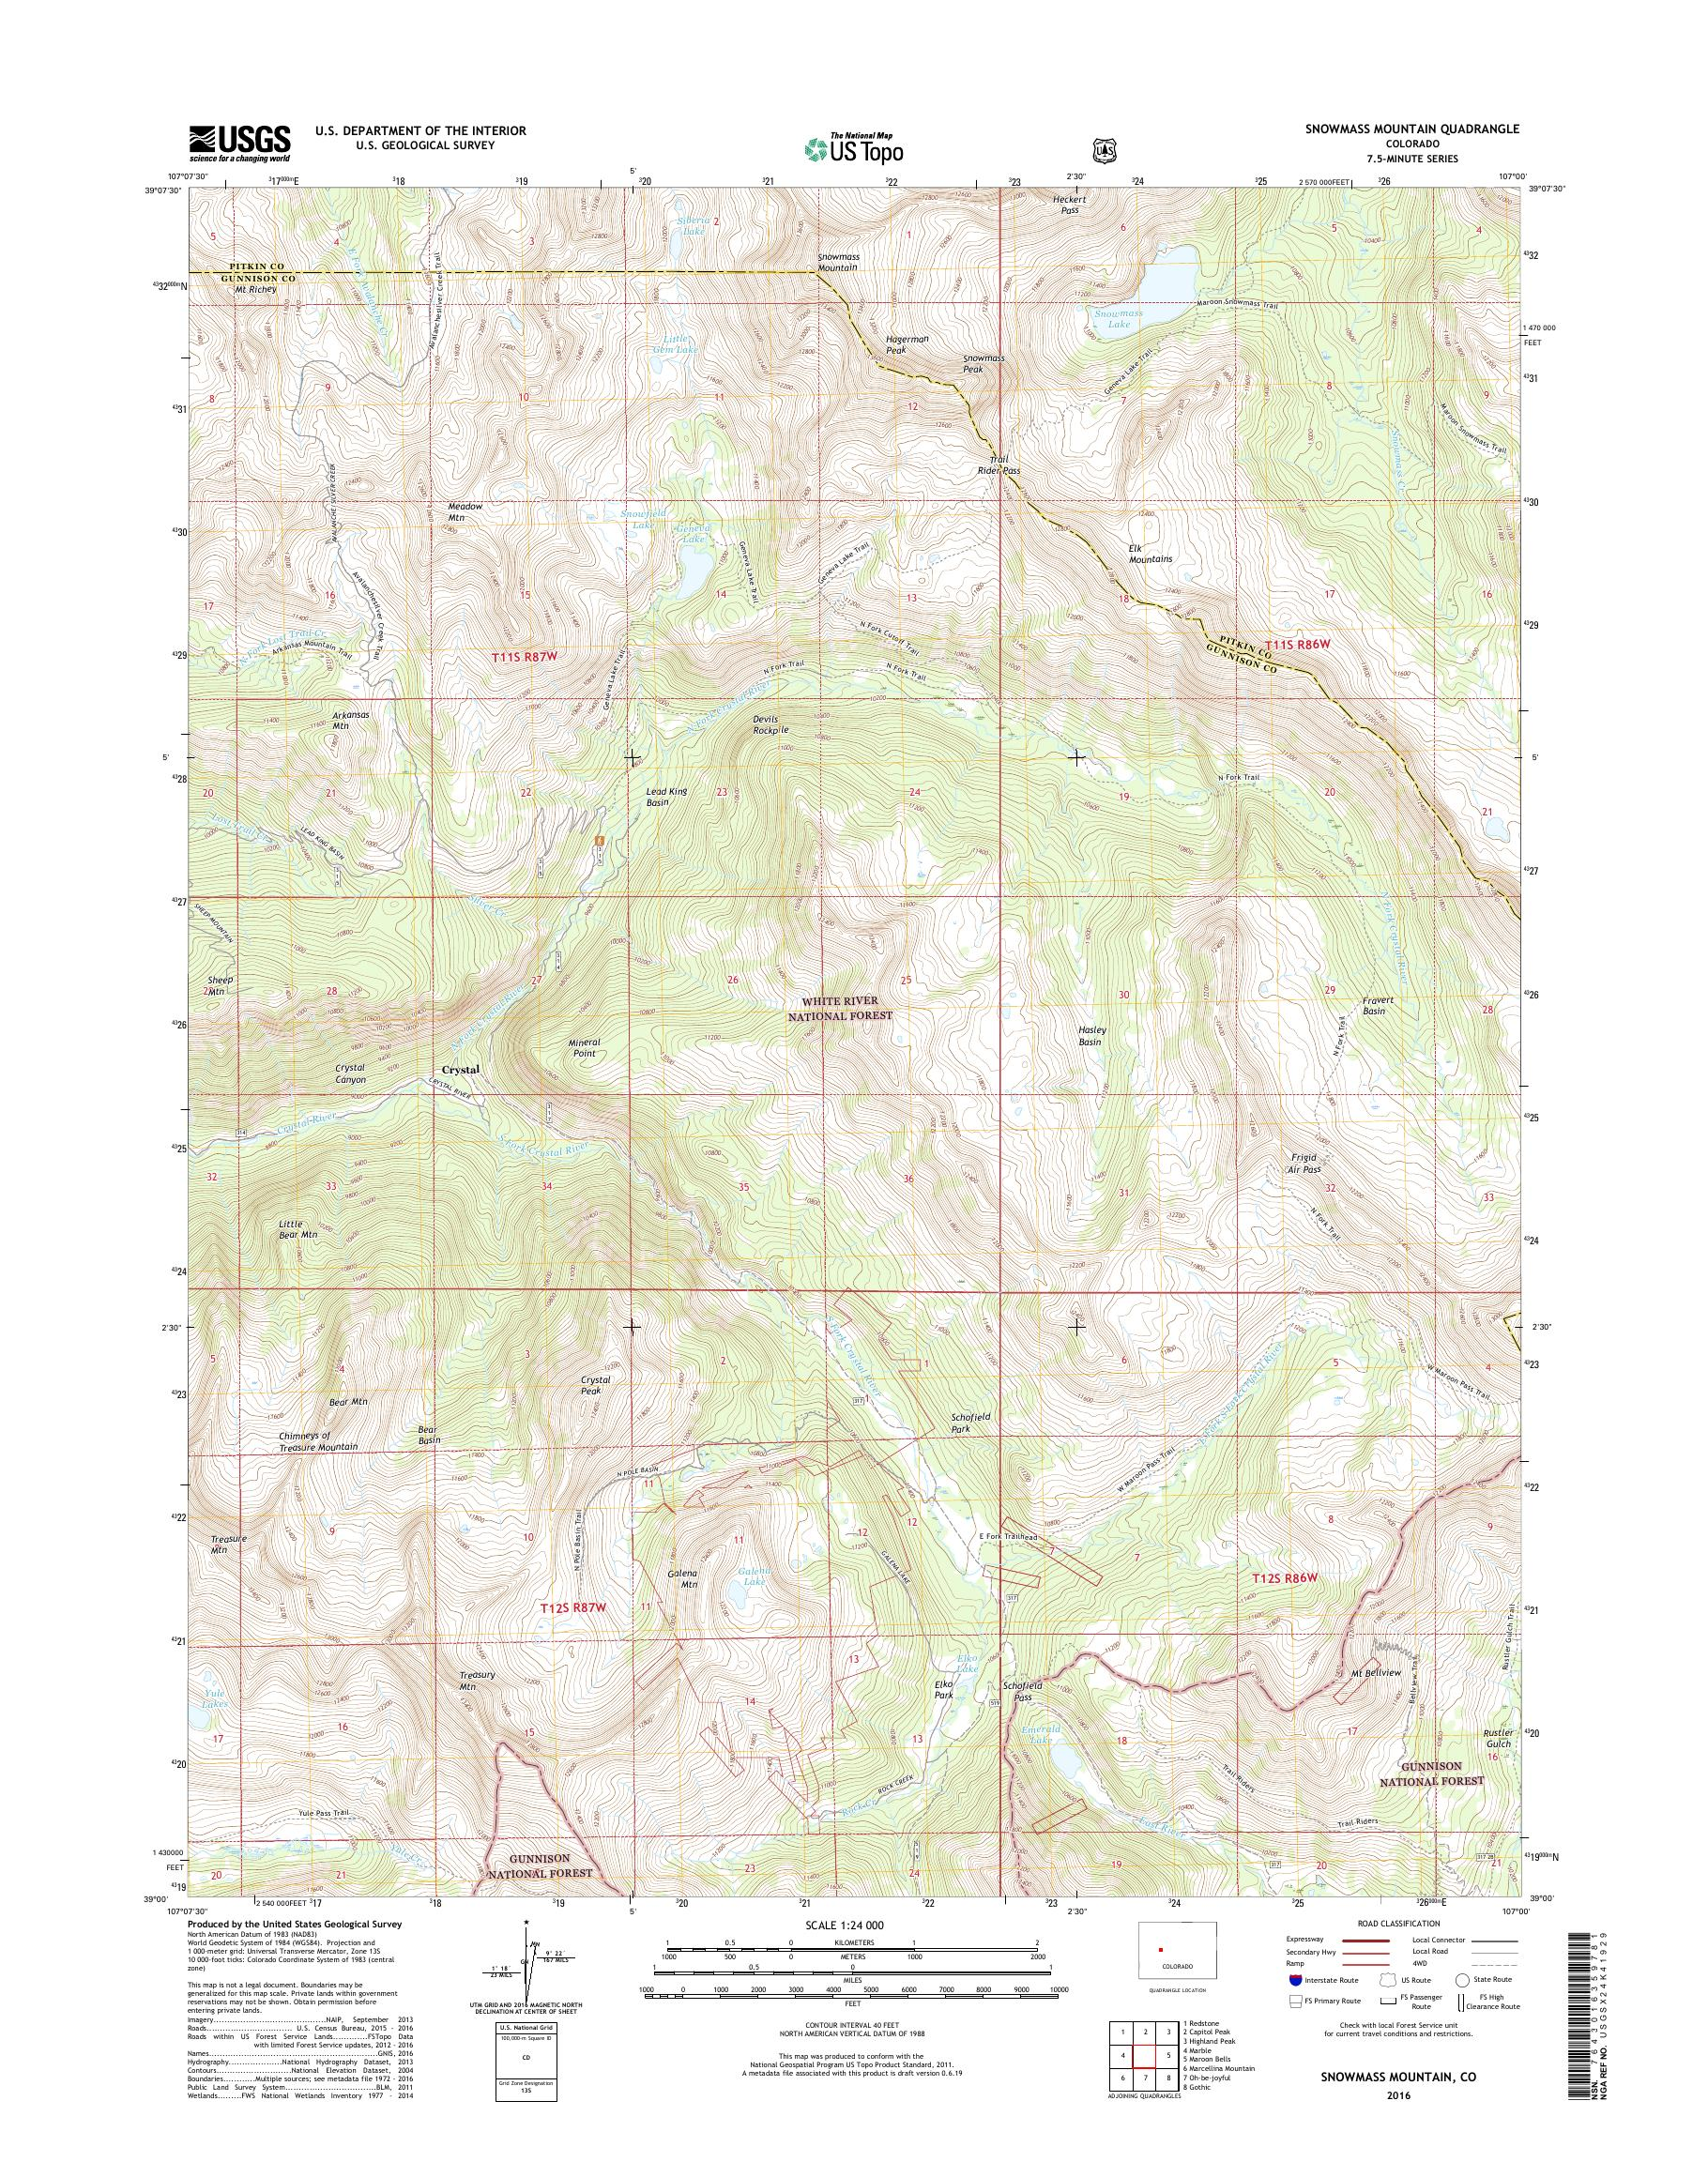
\includegraphics[width=1.1\textwidth]{figures/snowmass_topo.jpg}
\end{figure}
\end{problem}

\begin{problem}
Plot the following vector fields.
\begin{multicols}{2}
\begin{enumerate}[(a)]
    \item $\vecfieldU(x,y,z) = \begin{pmatrix} xyz \\ xyz \\ xyz \end{pmatrix}$.
    \item $\vecfieldV(x,y,z) = \begin{pmatrix} e^{x+y+z} \\ e^{x+y+z} \\ e^{x+y+z} \end{pmatrix}$.
    \item $\vecfieldW(x,y,z) = \begin{pmatrix} x \sin(y) \\ x \cos(y) \\ xz \end{pmatrix}$.
    \item $\forcevec(x,y,z) = \begin{pmatrix} 5 + yz \\ -5 -xz \\ xy \end{pmatrix}$.
\end{enumerate}
\end{multicols}
\end{problem}

\begin{problem}
Compute the divergence and curl of the vector fields in Problem 3.
\end{problem}

\begin{problem}
Given a function, a vector, and a point, compute the directional derivatives in the direction of the given vector at that point.
\begin{enumerate}[(a)]
    \item $f(x,y)=x^2/y$, $\vecu = 3\xhat -\yhat$, and $(x,y)=(2,2)$.
    \item $g(x,y,z)=x\cos(yz^2)$, $\vecv = \frac{1}{2}\xhat + \frac{1}{2} \yhat + \zhat$, and $(x,y,z)=(0,-1,2)$.
\end{enumerate}
\end{problem}

\begin{problem}
    Give a physical argument for why the field $\vecfieldU = \begin{pmatrix} 0 \\ x \\ 0 \end{pmatrix}$ has nonzero curl everywhere where $x\neq 0$. Reason why the direction of the curl is solely along the $z$-axis.  Do this \underline{without} computing the curl.
\end{problem}

\begin{problem}
    Give a physical argument why the field $\vecfieldV = \begin{pmatrix} x \\ 0 \\ 0 \end{pmatrix}$ has nonzero divergence everywhere where $x\neq 0$. Reason why the divergence is a scalar quantity as opposed to a vector quantity. Do this \underline{without} computing the curl.
\end{problem}

\begin{problem}
Compute the Laplacian of the following fields.
\begin{multicols}{2}
\begin{enumerate}[(a)]
    \item $f(x,y) = (x+y)^2$
    \item $g(x,y) = (x+y)e^{x^2+y^2}$.
    \item $\vecfieldU = \begin{pmatrix} \cos(x)\cos(y)\cos(z) \\ \sin(x)\sin(y)\sin(z) \\ xyz \end{pmatrix}$.
    \item $\vecfieldV = \begin{pmatrix} \frac{y}{z} \\ \frac{x}{z} \\ \frac{x}{y} \end{pmatrix}$.
\end{enumerate}
\end{multicols}
\end{problem}

\begin{problem}
    Suppose that $\vecfieldE = \grad \phi$ for some scalar field $\phi$ (as in the static Maxwell's equations).  Explain why if $\vecfieldE$ is divergence free (i.e., if $\grad \cdot \vecfieldE=0$) that $\veclaplace \vecfieldE = \zerovec$.
\end{problem}

\begin{problem}
    One of Maxwell's equations states for a magnetic field $\vecfieldB$ that
    \[
    \grad \cdot \vecfieldB = 0,
    \]
    is an identity.  Does this mean that $\veclaplace \vecfieldB = 0$? 
\end{problem}


\end{document}
